%! TEX root = ../../master.tex
\lecture[$\coNP$. Ellipsoid method. Separation vs. optimization.]{Di 03 May 2022}{Ellipsoid method}
\begin{definition}[$\NP$-hard]
    Consider an optimization problem $P$. We can't have $P \in \NP$, but because of \autoref{th:opt-dec-problem}
    we can introduce the notion to call $P$ \vocab[NP!hard]{$\NP$-hard}, if its decision variant is in $\NPC$.
\end{definition}
\begin{definition}[$\coNP$]
    We say \vocab[NP!co-NP]{$P \in \coNP$}, if we have a succinct certificate for verifying No-instances.
\end{definition}
\begin{example}
    Given a matrix $A$. We call it totally unimodular, if every square submatrix has determinant 0 or 1.
    Deciding if $A$ is totally unimodular is in $\coNP$, because giving a failing submatrix as a succinct certificate is easy.
\end{example}
\begin{theorem}
    The decision version of LP is in $\coNP$. \label{thm:LP-coNP}
\end{theorem}
\begin{proof}
    The answer to the decision problem is No iff
    \begin{enumerate}
        \item the system is infeasible, or
        \item the system is feasible, but the optimal cost is larger than the $z$ we want.
    \end{enumerate}
    Because both can be decided with the tools we have in polynomial time, LP is indeed in $\coNP$.
\end{proof}
\begin{definition}[$\coNP$-complete]
    Analoguous to \autoref{def:NPC}, we can also define \vocab[NP!coNP-complete]{$\coNP$-completeness}, or $\coNPC$, for the "most difficult" problem in $\coNP$.
\end{definition}
\begin{remark}
    It holds that $\coNPC \cap \NPC = \emptyset$, except $\pP = \NP$.
\end{remark}
\todo{images p np}
\begin{openquestion}
    Is $\pP = \NP$?
    \begin{multicols}{2}
        % \begin{figure}[htpb]
        \centering
        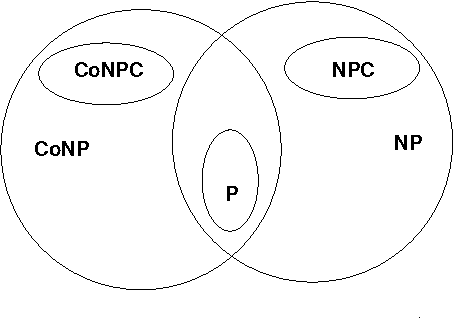
\includegraphics[width=.4\textwidth]{figures/np-not-p.png}\hfill
        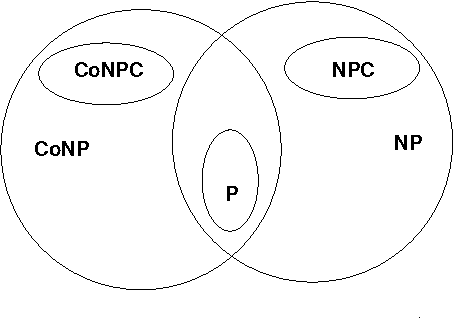
\includegraphics[width=.4\textwidth]{figures/np-not-p.png}\hfill
        % \caption{Picture of complexity if $\NP \neq P$}
        % \caption{Picture of complexity if $\NP = P$}
        % \end{figure}
    \end{multicols}

    % \begin{minipage}{\textwidth}
    %     \centering
    %     \begin{minipage}{0.45\textwidth}
    %         % 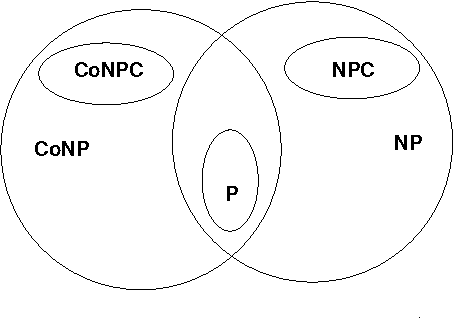
\includegraphics{figures/np-not-p.png}
    %         % https://www.semanticscholar.org/paper/Complexity-Theory-and-Np-completeness/a6894674c16ea11ab53e7f5567a645b9e0835afa/figure/4
    %         \captionof{figure}{Picture of complexity if $\NP \neq P$}
    %     \end{minipage}
    %     \begin{minipage}{0.45\textwidth}
    %         % 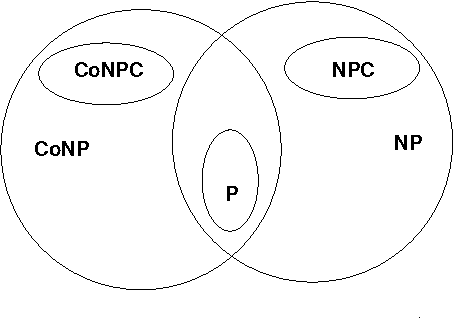
\includegraphics{figures/np-not-p.png}
    %     \end{minipage}
    %     % \captionof{figure}{Beispiele 'gleicher' metrischer Räume (homöomorph)}
    % \end{minipage}
\end{openquestion}
\begin{recall}[Ellipsoid Algorithm]
    As discussed in ADM1, the \vocab{ellipsoid method} can be used to determine feasibility of LPs in polynomial time.
    One could also call the ellipsoid method a fancy "$n$-dimensional binary search".
    A rough draft how the algorithm worked:
    \begin{enumerate}
        \item Reduce optimization version to decision version and introduce bound $L = mn \cdot \log(\text{max abs. data})$
        \item Volume-based argument: If the LP is feasible, there is a solution within the centered cube with length $2^L$.
        \item Volume is zero: Perturb the problem to $Ax \leq b + 2^{-L}$, which maintains feasibility, but now has positive volume.
    \end{enumerate}
    For details, refer to the slides from ADM1.
\end{recall}
\begin{remark}
    The key step of the ellipsoid method is to find a hyperplane that separated the current $x$ from the considered polyhedron.
    This is equivalent to solving the \vocab{separation problem} $\SEP$.
    Especially, iff $\SEP \in \pP$, then $\OPT \in \pP$.
\end{remark}
\begin{definition}
    Let $\mathcal{Q}$ be the class of full-dimensional polytopes with $0$ inside.
    We define the \vocab{polar} $Q^*$ for $Q \in \mathcal{Q}$ as
    \begin{align*}
        Q^* \coloneqq \{ y \in \realnum^n \mid y^Tx \leq 1 \forall x \in Q \}.
    \end{align*}
\end{definition}
\begin{theorem}
    Considering this class of polytopes, one can proove \cite[Ch.~4,~Thm.~4.22]{comb-optimization-korte}:
    \begin{enumerate}
        \item $Q^*$ is also a full-dimensional polytope with $0$.
        \item $(Q^*)^* = Q$
        \item $v$ is a vertex of $Q$ iff $v^Ty \leq 1$ is a facet of $Q^*$
    \end{enumerate}
\end{theorem}
\begin{theorem}
    Suppose we can solve $\OPT$ on $\mathcal{Q} \in \pP$ with algorithm $A$.
    Then we can use $A$ as an oracle to solve $\SEP$ on $\mathcal{Q}^*$ in polynomial time.
    \label{thm:sep-opt-lp}
\end{theorem}
\begin{proof}
    Suppose $Q^* \in \mathcal{Q}^*$, and we want to separate $y^0$.
    Use $A$ to solve $\OPT$ on $Q$ with objective function $\max (y^0)^Tx$ to get $x^* \in Q$.
    This yields two cases:
    \begin{itemize}
        \item $(y^0)^Tx^* \leq 1$: Then this holds for all $x \in Q$, and thus $y^0 \in Q^*$ by definition.
        \item $(y^0)^Tx^* > 1$: Consider hyperplane $(x^*)^Ty$. From $x^* \in Q$ it follows that
              for all $y \in Q^*$, that $(x^*)^Ty \leq 1$, but $(x^*)^Ty^0 > 1$. Thus, we found a separating hyperplane.
    \end{itemize}
\end{proof}
\begin{theorem}
    $\SEP \in \pP$ for $\mathcal{Q}$ iff $\OPT \in \pP$ for $\mathcal{Q}$
\end{theorem}
\begin{proof} Using what we proven so far:
    \begin{align*}
                                       & \OPT \in \pP \text{ for } \mathcal{Q}   &  & \overset{\ref{thm:sep-opt-lp}}{\IMP}  \SEP \in \pP \text{ for } \mathcal{Q}^*       \\
        \overset{\text{Ellips.}}{\IMP} & \OPT \in \pP \text{ for } \mathcal{Q}^* &  & \overset{\ref{thm:sep-opt-lp}}{\IMP}  \SEP \in \pP \text{ for } (\mathcal{Q}^*)^*=Q \\
        \overset{\text{Ellips.}}{\IMP} & \OPT \in \pP \text{ for } \mathcal{Q}
    \end{align*}
\end{proof}